\documentclass[letterpaper,11pt]{article}
\usepackage{graphicx}
\usepackage{listings}
\usepackage[super]{nth}
\usepackage[hyphens]{url}
\usepackage{hyperref}
\usepackage{amsmath}
\usepackage[makeroom]{cancel}
\usepackage[table]{xcolor}
\usepackage{comment}
\usepackage[space]{grffile}
\usepackage{csvsimple}
\usepackage{longtable}




\lstset{
	basicstyle=\footnotesize,
	breaklines=true,
}

\begin{document}

\begin{titlepage}

\begin{center}

\Huge{Assignment 8}

\Large{CS 532:  Introduction to Web Science}

\Large{Spring 2018}

\Large{Chandrasekhar Reddy Muthyala}


\end{center}

\end{titlepage}

\newpage


% =================================
% First question
% =================================
\section*{1}

\subsection*{Question}

\begin{verbatim}
(Spam classification using Naive Bayes classifier)
1. Create two datasets; the first called Testing, the second called Training. 
	
	The Training dataset should:
	a. consist of 10 text documents for email messages you consider spam
 (from your spam folder)
	b. consist of 10 text documents for email messages you consider not spam
 (from your inbox)

	The Testing dataset should:
	a. consist of 10 text documents for email messages you consider spam
 (from your spam folder)
	b. consist of 10 text documents for email messages you consider not spam 
(from your inbox)

	Upload your datasets on github
\end{verbatim}

\clearpage
\subsection*{Answer}
To solve this problem I have created two data sets as per the requirement. One is \textbf{Training dataset} and other is \textbf{ Testing dataset}. In both Training and Testing dataset, I added 10 spam and 10 non spam emails from spam folder and inbox respectively. 
\begin{figure}[h]
\centering
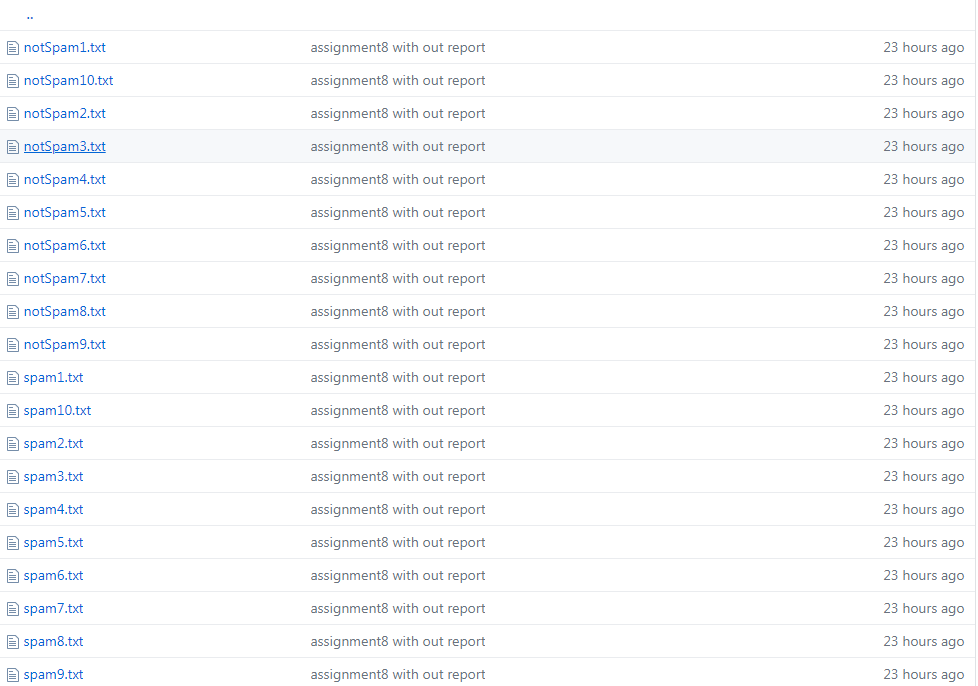
\includegraphics[width=\textwidth]{trainDataSetImage.png}
\caption{ Training dataset  image }
\label{fig:q2followers}
\end{figure}

\begin{figure}[h]
\centering
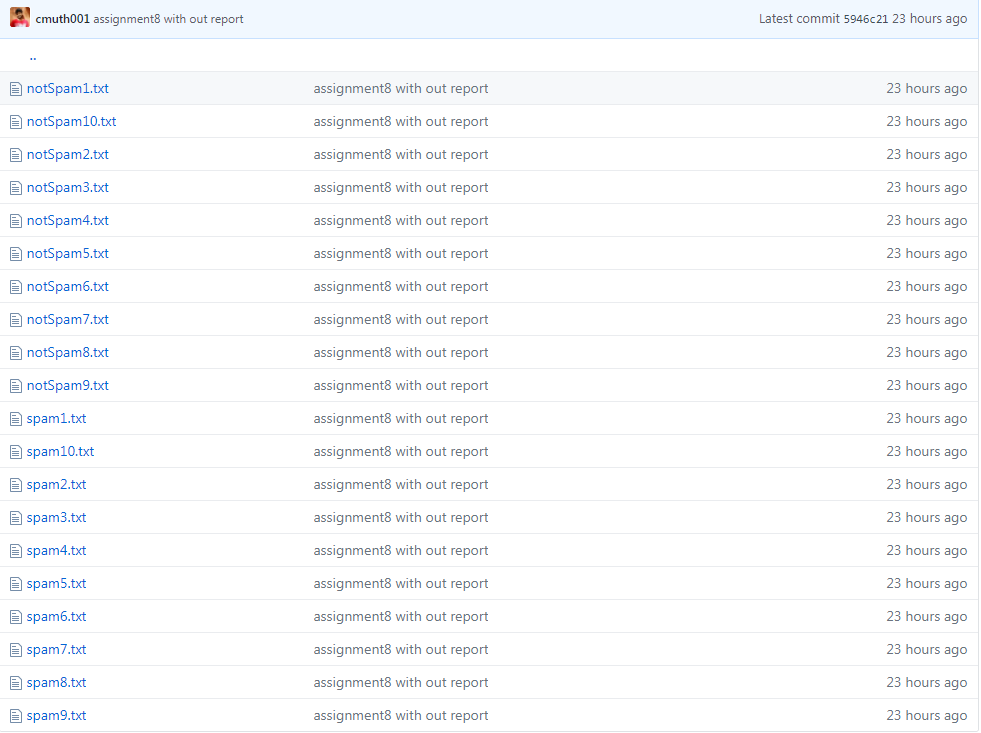
\includegraphics[width=\textwidth]{testDataSetImage.png}
\caption{ Testing dataset  image}
\label{fig:q2followers}
\end{figure}

\clearpage

% =================================
% Second question
% =================================

\section*{2}

\subsection*{Question}

\begin{verbatim}
2. Using the PCI book modified docclass.py code and test.py 
(see Slack assignment-8 channel)
Use your Training dataset to train the Naive Bayes classifier
 ( e.g., docclass.spamTrain() )
Use your Testing dataset to test (test.py)
 the Naive Bayes classifier and report the classification results.
\end{verbatim}

\subsection*{Answer}

To solve this Spam classification using Naive Bayes classifier I have gone through class note and  few other articles to understand how it will classify email  whether  spam or not. This classifier aggregates information using conditional probability. I have modified \textbf{docclass.py} code and\textbf{ test.py} to get the result.

In \textbf{docclass.py}  I added one more function checkSpamOrNot to train my dataset. In this function I am looping all the 10 spam and 10 non spam emails from train dataset. Read each text file and pass that text to train function for training. 

To find spam or not spam email I have used \textbf{test.py} and modified as per the requirement. In order to calculate confusion matrix I used one variable “output” which will store all the True positives, True negatives, False positives and False negatives. Looping all the 10 spam and 10 non spam emails from test dataset to classify each email.



\textbf{True positives}: “not spam email” classifies as “not spam email”

\textbf{True negatives}: “spam email” classifies as “spam email”

\textbf{False positives}: “spam email” classifies as “not spam email”

\textbf{False negatives}: “not spam email” classifies as “spam email”





The test dataset results as given below:

\textbf{True positives}: 7

\textbf{True negatives}: 10

\textbf{False positives}: 0

\textbf{False negatives}: 3



 \begin{figure}[h]
 \centering
 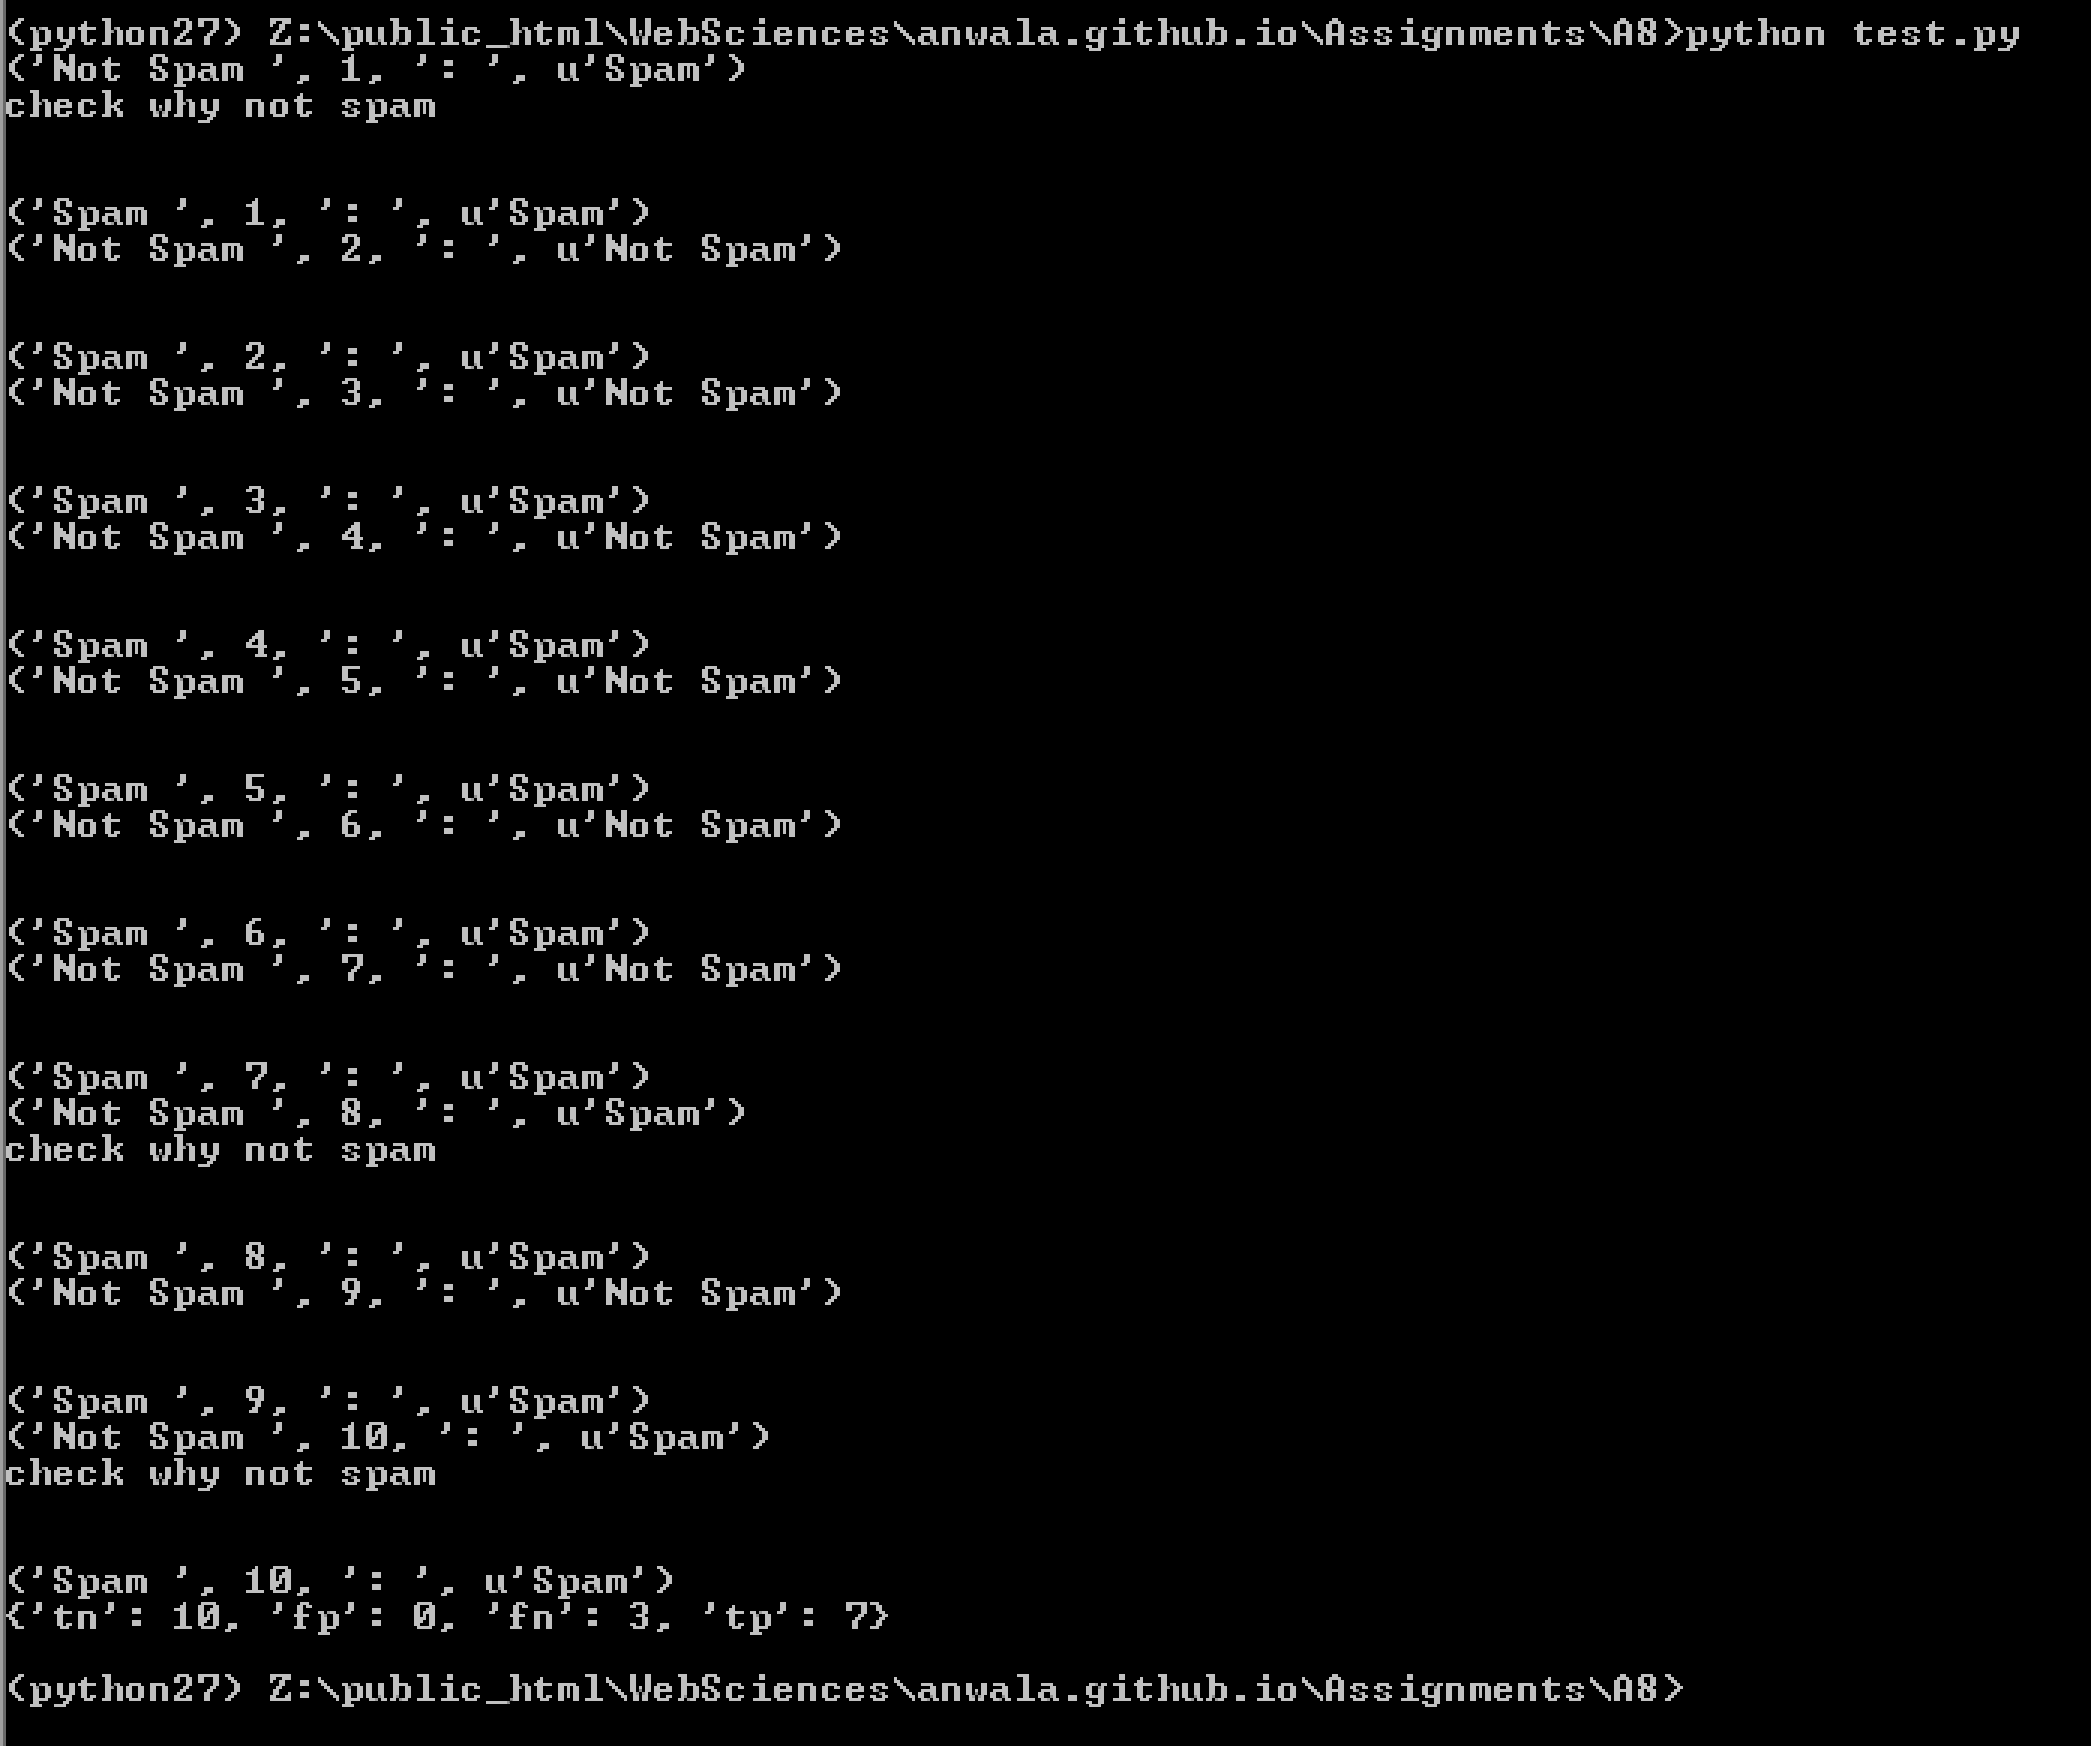
\includegraphics[scale=0.26]{output}
 \caption{Out put of my test dataset}
 \label{fig:dendro}
 \end{figure}
\clearpage
\lstinputlisting[frame=single,caption={Python script for training and classify dataset},label=lst:createClusters,captionpos=b,numbers=left,showspaces=false,showstringspaces=false,basicstyle=\footnotesize]{docclass.py}

\lstinputlisting[frame=single,caption={Python script to  classify test dataset },label=lst:createClusters,captionpos=b,numbers=left,showspaces=false,showstringspaces=false,basicstyle=\footnotesize]{test.py}


\clearpage

% =================================
% 3rd question
% =================================

\section*{3}

\subsection*{Question}

\begin{verbatim}
3. Draw a confusion matrix for your classification results
(see: https://en.wikipedia.org/wiki/Confusion_matrix)
\end{verbatim}

\subsection*{Answer}

The below confusion matrix is drawn using 2nd problem output.
\begin{table}[htb]
\begin{tabular}{ | c | c | c | }
\hline
\textbf{} & \textbf{Not Spam} & \textbf{spam}  \\
\hline
\textbf{Not Spam} &True Positives - 7  & False Negative -  3 \\
\hline
\textbf{spam} &False Positives - 0 & True Negatives -10 \\
\hline
\end{tabular}
\caption{confusion matrix}
\label{table:q1user1}
\end{table}
Out of all the emails in the test dataset there were 3 not spam emails classified as spam. I think those 3 not spam emails contain mostly HTML tags and my spam traing dataset also contain HTML tags so I feel the probability of  spam email content is high in those 3 not spam email.

\clearpage

% =================================
% 4th question
% =================================

\section*{4}

\subsection*{Question}

\begin{verbatim}
4. Report the precision and accuracy scores of your classification results
(see: https://en.wikipedia.org/wiki/Precision_and_recall)
\end{verbatim}

\subsection*{Answer}

	By using True positives, True negatives, False positives and False negatives I calculated  precision and accuracy scores.
	\[Precision 
	= \dfrac{tp}{tp\texttt{+}fp}
  	= \dfrac{7}{7\texttt{+}0}
	=1
\]
\[Recall  
 	 = \dfrac{tp}{tp\texttt{+}fn}
  	= \dfrac{7}{7\texttt{+}3}	
	=0.7
\]

\clearpage


% =================================
% Bibliography
% =================================

\begin{thebibliography}{9}
\bibitem{}
\url{https://en.wikipedia.org/wiki/Precision_and_recall}.
\bibitem{}
\url{https://en.wikipedia.org/wiki/Confusion_matrix}.
\bibitem{}
 \url{http://scikit-learn.org/stable/modules/naive_bayes.html}.
\bibitem{}
\url{https://machinelearningmastery.com/naive-bayes-classifier-scratch-python/}
\bibitem{}
 \url{https://github.com/arthur-e/Programming-Collective-Intelligence}.
\end{thebibliography}

\end{document}